%KECReportFormat.tex
%%%%%%%%%%%%%%%%%%%%%%%%%%%%%%%%%%%%%%%%%%%%%%%%%%%%%%%%%%%%%%%%%%%%%%%%%%%
%DO NOT MAKE CHANGES IN THIS FILE

\documentclass[12pt, a4paper]{report}
\usepackage[left = 1.5in, right = 1in, top = 1in, bottom = 1in]{geometry}%for margin
\usepackage{amsfonts, amsmath, amssymb} %for mathematical equations
\usepackage{graphicx} %for images
\usepackage{times} %font Times New Roman Font
\usepackage{float} %required if you use H(strictly here) position for floats
\usepackage[skip = 8pt,tableposition=top, figureposition=bottom]{caption}%adjust spacing of captions and specify where captions are
\usepackage{hyperref} % for easy Navigation in document, also puts links in TOC, LOF, LOT...
\usepackage{setspace} %to change line spacing in some portion \singlespacing \onehalfspacing \doublespacing
\usepackage{acro} %for List of Abbrreviation and Symbol
\acsetup{first-style = short} % set to display only short form on the command \ac{}

%packages required for complex tables
\usepackage{bigstrut} 
\usepackage{multirow}

\renewcommand{\contentsname}{Table of Contents} %Change TOC Heading ... default is "Contents" 

\parindent 0pt	%removes the indent in paragraph
\setlength{\parskip}{18pt}	%for paragraph spacing
\renewcommand{\baselinestretch}{1.5}   %Line Spacing = 1.5 line-spaces

%to reduce spacing in sections
\usepackage{titlesec}
\titlespacing*{\section}{0pt}{0pt}{0pt} %left, top, bottom spacings
\titlespacing*{\subsection}{0pt}{0pt}{0pt}
\titlespacing*{\subsubsection}{0pt}{0pt}{0pt}
\titlespacing*{\paragraph}{0pt}{0pt}{0pt}
\titlespacing*{\subparagraph}{0pt}{0pt}{0pt}

%adjust fontsizes\ of sections
\titleformat*{\section}{\fontsize{14pt}{18pt}\bfseries}
\titleformat*{\subsection}{\fontsize{13pt}{18pt}\bfseries}
\titleformat*{\subsubsection}{\fontsize{12pt}{18pt}\bfseries}
\titleformat*{\paragraph}{\fontsize{12pt}{18pt}\bfseries}
\titleformat*{\subparagraph}{\fontsize{12pt}{18pt}\bfseries}

%to reduce separation between points in list
\usepackage{enumitem}
\setlist[enumerate]{nosep} % no separation between items in enumerate
\setlist[itemize]{nosep} % no separation between items in itemize
%use \vspace{-18pt} before list to reduce paragraph spacing between list and preceeding paragraph.

%Changes for Chapter Heading Spacing and formats for numbered chapters
\makeatletter
\def\@makechapterhead#1{%
  %\vspace*{50pt}%
  {  \MakeUppercase{\ifnum \c@secnumdepth >\m@ne
        \fontsize{16pt}{1}\bfseries \@chapapp \space \thechapter\vspace{5pt}\\
    \fi
    \interlinepenalty\@M
     \bfseries #1}\par\nobreak
    %\vskip 0pt
  }}
\makeatother

%%%%%%%%%%%%%%%%%%%%%%%%%%%%%%%%%%%%%%%%%%%%%%%%%%%%%%%%%%%
%to adjust Heading spacings and fonts For unnumbered chapters, TOC, LOF ...
\makeatletter
% Redefine the \chapter* header macro to remove vertical space
\def\@makeschapterhead#1{%
  %\vspace*{50\p@}% Remove the vertical space
  {\newpage \parindent \z@ \raggedright
    \normalfont
    \interlinepenalty\@M
    \center \fontsize{16pt}{1} \bfseries \MakeUppercase{#1}\par\nobreak
    %\vskip 18\p@ % adjust space after heading 18pt
  }}
\makeatother 
%%%%%%%%%%%%%%%%%%%%%%%%%%%%%%%%%%%%%%%%%%%%%%%%%%%%%%%%%%%

%%%%%%%%%%%%%%%%%%%%%%%%%%%%%%%%%%%%%%%%%%%%%%%%%%%%%%%%%%%%%%%%%%%%%%%%%%%
% newcommand for generating Cover Page
\newcommand{\KECcoverpage}
{
\begin{titlepage}
\begin{center}
\Large{\textbf{KANTIPUR ENGINEERING COLLEGE}}\\
\large{\textbf{(Affiliated to Tribhuvan University)}}\\
\large{\textbf{Dhapakhel, Lalitpur}}\\
\vfill	%vertically fill the space 
\begin{figure}[h] % h: put logo "here"
\begin{center}

\includegraphics[width=25mm, height = 25mm]{images/logo.png}
\end{center}
\end{figure}

\large{\textbf{[Subject Code: \subCode]}}\\ %Change This Line
\large{\textbf{A \MakeUppercase{\project} \MakeUppercase{\doc} ON}}\\ %Change This Line
\Large{\textbf{\MakeUppercase{\projectTitle}}}\\

\vfill	%vertically fill the space 
\large{\textbf{Submitted by:}}\\
\large{\textbf{\submittedBy}}\\
\vfill	%vertically fill the space 
\textbf{A \MakeUppercase{\project} SUBMITTED IN PARTIAL FULFILLMENT OF THE REQUIREMENT FOR THE DEGREE OF \MakeUppercase{\degree}}\\

\vfill	%vertically fill the space 
\large{\textbf{Submitted to:}}\\
\large{\textbf{\submittedTo}}\\
\vfill
\large{\textbf{\defMonth, \defYear}}
\pagebreak
\end{center}
\end{titlepage}
}
%%%%%%%%%%%%%%%%%%%%%%%%%%%%%%%%%%%%%%%%%%%%%%%%%%%%%%%%%%%%%%%%%%%%%%%
% newcommand for generating Cover Page
%Title Page
\newcommand{\KECtitlepage}
{
\begin{titlepage}
\begin{center}
\Large{\textbf{\MakeUppercase{\projectTitle}}}\\

\vfill	%vertically fill the space 

\large{\textbf{Submitted by:}}\\
\large{\textbf{\submittedBy}}\\


\ifhassupervisor % Displays Supervisor name only if \hassupervisortrue
	\vfill	%vertically fill the space 
	\large{\textbf{Supervised by:}}\\
	\large{\textbf{\supervisor}}\\
	\large{\textbf{\degSup}}\\
\fi

\vfill	%vertically fill the space 
\textbf{A \MakeUppercase{\project} SUBMITTED IN PARTIAL FULFILLMENT OF THE REQUIREMENT FOR THE DEGREE OF \MakeUppercase{\degree}}\\

\vfill	%vertically fill the space 
\large{\textbf{Submitted to:}}\\
\large{\textbf{\submittedTo}}\\
\large{\textbf{Kantipur Engineering College}}\\
\large{\textbf{Dhapakhel, Lalitpur}}\\

\vfill
\large{\textbf{\defMonth, \defYear}}
\thispagestyle{empty}\\ %to remove page number
\pagebreak
\end{center}
\end{titlepage}
}
%%%%%%%%%%%%%%%%%%%%%%%%%%%%%%%%%%%%%%%%%%%%%%%%%%%%%%%%%%%%%%%%%%%%%%
%command for copyright page
\newcommand{\KECcopyright}
{
\chapter*{Copyright}%Required only for Final Defense of Major Project
\addcontentsline{toc}{chapter}{Copyright}
The author has agreed that the library, Kantipur Engineering Collage, may make this report freely available for inspection. Moreover the author has agreed that permission for extensive copying of this report for scholarly purpose may be granted by the supervisor(s), who supervised the project work recorded herein or, in their absence, by the Head of the Department wherein this project was done. It is understood that due recognition will be given to the author of this report and to the \submittedTo, Kantipur Engineering College in any use of the material of this report. Copying or publication or other use of this report for financial gain without approval of the \submittedTo, Kantipur Engineering College and author’s written permission is prohibited.\par Request for permission to copy or to make any other use of the material in this report in whole or in part should be addressed to:

Head\\
\submittedTo\\
Kantipur Engineering College\\
Dhapakhel, Lalitpur\\
Nepal
}
%%%%%%%%%%%%%%%%%%%%%%%%%%%%%%%%%%%%%%%%%%%%%%%%%%%%%%%%%%%%%%%%%%%%%%
%command for Approval Letter
\newcommand{\KECapproval}
{
\chapter*{Kantipur Engineering College
\vskip -10pt}%Required only for Final Defense of Major Project
\begin{center}
\fontsize{12.8pt}{1} %size decreaced to adjust department name in single line
\textbf{
\MakeUppercase{\submittedTo}\\ %for department name
}
\vskip 10pt
\fontsize{16pt}{1}
\textbf{APPROVAL LETTER}
\end{center}
\vskip -16pt
\addcontentsline{toc}{chapter}{Approval Letter}%
The undersigned certify that they have read and recommended to the Institute of Engineering for acceptance, a project report entitled "\projectTitle " submitted by \\
\submittedBy \\
in partial fulfillment for the degree of \degree. \par
{\vspace{25pt}
..........................................\\
Supervisor\\
\supervisor \\
\degSup\\
\vspace{25pt}\\
..........................................\\
External Examiner\\
\external\\
\degExternal\\
\vspace{25pt}\\
..........................................\\
\hod\\
Head of Department\\
\submittedTo
\vspace{10pt}\\
Date: \defMonth\space\defDay ,\space \defYear
\singlespacing\par
} %single spacing for the texts inside {}
}

%command for list of abbreviations
\newcommand{\KECloa}
{
\chapter*{List of Abbreviations}
\addcontentsline{toc}{chapter}{List of Abbreviations}
\vskip -42pt % to reduce space due to invisivle acronym class name
{
\singlespacing
\printacronyms[include-classes=abbr, name= ]
}

}

%command for list of symbols
\newcommand{\KEClos}
{
\chapter*{List of Symbols}
\addcontentsline{toc}{chapter}{List of Symbols}
\vskip -42pt % to reduce space due to invisivle acronym class name{
{
\singlespacing
\printacronyms[include-classes=symbol, name= ]
}
}

%command to adjust toc, lof, lot spacing
\newcommand{\KECadjusttocspacings}
{
\parskip 0pt % to remove paragraph spacing in TOC, LOF ...
\renewcommand{\baselinestretch}{0.1} % to adjust line spacing in toc
\newcommand*{\noaddvspace}{\renewcommand*{\addvspace}[1]{}}
\addtocontents{lof}{\protect\noaddvspace} %remove extra vertical space in LOF
\addtocontents{lot}{\protect\noaddvspace} %remove extra vertical space in LOT
} %includes the file KecReportFormat.tex that include all necessary formattings
%\usepackage[first-style=long]{acro}

%%%%%%%%%%%%%%%%%%%%%%%%%%%%%%%%%%%%%%%%%%%%%%%%%%%%%%%%%%%%%%%%%%%%%%%%%%%
%Define Macros for Details of your Project
\newcommand{\project}{Major Project } %Specify "Major Project" or "Minor Project"
\newcommand{\projectTitle}{NEPALI SPEECH RECOGNITION USING BiLSTM and ResNet} %specify "Title" of Your Project
\newcommand{\doc}{Mid-Term Report} % specify the document you are preparing eg. "Proposal", "Mid-Term Report" or "Final Report"32
% Note that You have to sibmit "Final Report" for Pre-final defense as well.
\newcommand{\subCode}{CT707} %specify Subject of Your Project
\newcommand{\degree}{Bachelor in Computer Engineering} %specify your degree
\newcommand{\submittedBy}%Specify Names and Roll/Symbol Numbers of the Project Group Members
{
%Edit Member Names and Roll/Symbol No. and adjust width (\makebox[width]) if necessary 
\makebox[7cm]{Ankit Kafle \hfill [KAN076BCT012]}\\
\makebox[7cm]{Dikshyanta Giri \hfill [KAN076BCT026]}\\
\makebox[7cm]{Jenith Rajlawat \hfill [KAN076BCT034]}\\
\makebox[7cm]{Nawaraj Shah \hfill [KAN076BCT044]}
%\makebox[9cm]{Member Name \hfill [Roll/Symbol No.]}\\
} % Note that You must write your "Symbol Numbers"(Exam Roll Numbers) for Final Defenses

\newcommand{\submittedTo}{Department of Computer and Electronics Engineering} %specify your department
\newcommand{\hod}{Er. Rabindra Khati} %specify Head ot the department
\newcommand{\defYear}{2023} %Defense Year
\newcommand{\defMonth}{August} %Defense Month- January, February, ...
\newcommand{\defDay}{1} %specify Defense Day- 1, 2, ...

\newif\ifhassupervisor
\hassupervisorfalse % to display supervisor name use command- \hassupervisortrue
 
\newcommand{\supervisor}{Supervisor's Name} % Specify Name of Supervisor for Major Project
\newcommand{\degSup}{Supervisor's Designation\\Second Line of Designation (if required)} %Specify Designation of Supervisor for Major Project, use multiple lines (\\) if necessary
\newcommand{\external}{External's Name} %Specify Name of External for Major Project (Required for Black Book)
\newcommand{\degExternal}{External's Designation\\Second Line of Designation (if required)} %Specify Name of External for Major Project (Required for Black Book) , use multiple lines (\\) if necessary


%%%%%%%%%%%%%%%%%%%%%%%%%%%%%%%%%%%%%%%%%%%%%%%%%%%%%%%%%%%%%%%%%%%%%%%%%%%

%%%%%%%%%%%%%%%%%%%%%%%%%%%%%%%%%%%%%%%%%%%%%%%%%%%%%%%%%%%%%%%%%%%%%%%%%%%
%Define Abberviations and Symbols
% NOTE that Only those Abberviations and Symbols that are included in document(using command \ac{}) will be displayed in the List of Abberviations and Symbols.

%class 'abbr': for List of Abbreviations
\DeclareAcronym{OCR}{
    short = OCR,
    long = Optical Character Recognition,
    tag = abbr
}
\DeclareAcronym{LPR}{
    short = LPR,
    long = License Plate Recognition,
    tag = abbr
}
\DeclareAcronym{KNN}{ 
  short = KNN ,
  long  = K-Nearest Neighbor ,
  tag = abbr
}% declares acronym named "UN". Use \ac{UN} for short and \acl{UN} for long form. 

\DeclareAcronym{TTS}{
  short = TTS ,
  long  = Text To Speech ,
  tag = abbr
}
\DeclareAcronym{CNN}{
  short = CNN ,
  long  = Convolutional Neural Network ,
  tag = abbr
}
\DeclareAcronym{YOLO}{
    short=YOLO,
    long = You Only Look Once,
    tag= abbr,
}
\DeclareAcronym{LP}{
    short = LP,
    long = License Plate,
   	tag = abbr,
    }
\DeclareAcronym{GPU}{
    short = GPU,
    long = Graphics Processing Unit,
    tag = abbr
}
\DeclareAcronym{ANPR}{
    short = ANPR,
    long = Automatic Number Plate Recognition,
    tag = abbr
}
\DeclareAcronym{API}{
    short = API,
    long = Application Programming Interface,
    tag = abbr
}
\DeclareAcronym{BERT}{
    short = BERT,
    long = Bidirectional Encoder Representations from Transformers,
    tag = abbr
}
\DeclareAcronym{IAST}{
    short = IAST,
    long =  International Alphabet of Sanskrit Transliteration ,
    tag = abbr
}
\DeclareAcronym{UML}{
    short = UML,
    long =  Unified Modelling Language ,
    tag = abbr
}
\DeclareAcronym{ITRANS}{
    short = ITRANS,
    long = Indian Language Transliteration,
    tag = abbr
}
%%%%%%%%%%%%%%%%%%%%%%%%%%%%%%%%%%%%%%%%%%%%%%%%%%%%%%%%%%%%%%%%%
% class `symbol': for List of Symbols
\DeclareAcronym{transparencyFactor}{
  short = \ensuremath{\alpha} ,
  long  = Transparency Factor ,
  sort  = Transparency Factor , % string to compare for sorting symbols... default string is the acronym name -"transparencyFactor"
  tag = symbol
}% declares acronym named "transparencyFactor". Use \ac{UN} for short and \acl{UN} for long form.

\DeclareAcronym{areaOfTriangle}{
  short = \ensuremath{a} , % use \ensuremath{a} instead of $a$
  long  = Area of Triangle ,
  sort  = Area of Triangle , % string to compare for sorting symbols
  tag = symbol
}
%%%%%%%%%%%%%%%%%%%%%%%%%%%%%%%%%%%%%%%%%%%%%%%%%%%%%%%%%%%%%%%%%%%%%%%%%%%%%%%%%%%%%%%%%%%%%%%%%%%%

%%%%%%%%%%%%%%%%%%%%%%%%%%%%%%%%%%%%%%%%%%%%%%%%%%%%%%%%%%%%%%%%%%%%%%%%%%
%The Document
\begin{document}


\KECcoverpage % command defined in KECReportFormat
\KECtitlepage % command defined in KECReportFormat

\pagenumbering{roman} % starts pagenumberins in Roman numerals i, ii, ...



 



%\chapter*{Abstract} % The summary of your report
%\addcontentsline{toc}{chapter}{Abstract}%to include this chapter in TOC 
%With the advancement in Machine Learning models, machines are being made capable of doing tasks that otherwise require human intelligence. Artificial Intelligence (AI) technology has paved the way for the development of AI voice assistants, transforming the way humans interact with computers and digital devices. In today’s world, Automatic Speech Recognition(ASR) can be an ideal thing to do with the development of technology. So our proposed system Nepali Voice Assistant is a voice assistant which recognizes Nepali speech, processes it and then executes the required operation. Our system aims to develop a Nepali AI voice assistant by leveraging a combination of advanced neural network models. The process begins with data cleaning, where we remove (audio, text) pairs that include Devanagari numeric transcriptions, ensuring a clean and relevant dataset. Next, we extract Mel-frequency cepstral coefficients (MFCCs) from the preprocessed audio data. These MFCCs capture the spectral characteristics of Nepali speech and serve as essential input features for our neural network. To design an optimal model  Convolutional Neural Networks (CNN), Residual Networks (ResNet), and Bidirectional Long Short-Term Memory (BiLSTM) layers are used. The CNN layers excel at extracting local patterns and spatial features from the MFCC input, while the ResNet layers help capture deeper representations for enhanced performance. The BiLSTM layers are employed to model the temporal dependencies present within the speech data. Connectionist Temporal Classification (CTC) loss function is used to enable s sequence-to-sequence mapping by aligning the input speech with the corresponding text outputs. 


%\par
%\textbf{\textit{Keywords$-$}}{\textit{ Artificial Intelligence,}}{\textit{ Automatic Speech Recognition,}} {\textit{  Convolutional Neural Networks,}}{\textit{  Gated Recurrent Units,}}{\textit{Connectionist Temporal Classification,}}{\textit{  Mel-frequency cepstral coefficients,}}{\textit{ Recurrent Neural Network,}}{\textit{ Residual Networks,}}{\textit{ Bidirectional Long Short-Term Memory.}}

\par
%to display members name under Acknowledgement
%\begin{flushright}
%\vskip -20pt
%\setstretch{1.2}
%\submittedBy
%\end{flushright}

%to adjust spacings for TOC, LOF, LOT
{
%%%%%%%%%%%%%%%%%%%%%%%%%%%%%%%%%%%%%%%%%%%%%%%%%%%%%%%%%%%%%%%%%%%%%%%%%%%
%TOC, LOF and LOT
\KECadjusttocspacings % defined in KECReportFormat.tex to adjust spacings
\makeatletter
% to add vskip of 18 point which is reduced when parskip is set to 0 in \LECadjustspacings
\def\@makeschapterhead#1{%
  %\vspace*{50\p@}% Remove the vertical space
  {\newpage \parindent \z@ \raggedright
    \normalfont
    \interlinepenalty\@M
    \center \fontsize{16pt}{1} \bfseries \MakeUppercase{#1}\par\nobreak
    \vskip 18\p@ % adjust space after heading 18pt
  }}
\makeatother 
\setcounter{secnumdepth}{5}

\tableofcontents % prints table of contents
\listoffigures % prints list of figures
\addcontentsline{toc}{chapter}{List of figures}

%\addcontentsline{toc}{chapter}{Acknowledgement}

\chapter*{List of Abbreviations}
	AI: Artificial Intelligence\\
	ASR: Automatic Speech Recognition\\
	BILSTM: Bidirectional Long Short-Term Memory\\
	CNN: Convolutional Neural Network \\
	CTC: Connectionist Temporal Classification\\
	E2E: End-To-End\\
	GRU: Gated Recurrent Units\\
	MFCCs:  Mel-frequency cepstral coefficients\\
	RESNET: Residual Networks\\	
	RNN: Recurrent Neural Network 
	
	
	

\addcontentsline{toc}{chapter}{List of abbreviations}	
	
	
%\listoftables % prints list of table
}
%%%%%%%%%%%%%%%%%%%%%%%%%%%%%%%%%%%%%%%%%%%%%%%%%%%%%%%%%%%%%%%%%%%%%%%%%%%

%comment this chapter if you don't have List of Abbreviations
%\KECloa % defined in KECReportFormat

%comment this chapter if you don't have List of Symbols
%\KEClos % defined in KECReportFormat

\newpage
\pagenumbering{arabic} % starts pagenumbering in arabic numerals

\chapter{Introduction}
\section{Background}\label{sec:bkgrnd}%label your section if you require to refer them somewhere else in your document.
Speaking and writing are the two important things that help us to communicate among us. Deficient either in writing or speaking affects our daily activities. Most of the people in rural areas are able to speak properly but not able to write properly. Most communication technology (gadgets, mobiles, computers, etc) needs text as an input for their operation. To be familiar with the technology like Automatic Speech Recognition (ASR) can play a significant role \cite{bhatta2020nepali}. Automatic Speech Recognition (ASR) is a technology that enables machines to convert spoken language into written text. It has evolved significantly over the years and has found applications in various fields, including telecommunications, transcription services, virtual assistants, voice-controlled systems, and more. The development of ASR systems has revolutionized human-computer interaction, allowing for more natural and intuitive communication.

Automatic Speech Recognition (ASR) is essential due to several significant reasons. Firstly, it enables a natural and intuitive means of interaction between humans and machines. By speaking commands or queries instead of typing or pressing buttons, users can engage with technology more seamlessly, providing convenience and accessibility. ASR also plays a crucial role in making digital content and services accessible to individuals with hearing or speech impairments, allowing them to participate in conversations, consume media, and access information through captioning and transcription services. Furthermore, ASR systems that support multiple languages foster effective communication across language barriers, promoting global connectivity and understanding. ASR significantly enhances efficiency and productivity in various domains, automating tasks like transcription and streamlining workflows. It forms the backbone of voice-controlled systems, enabling virtual assistants to accurately understand and execute user instructions. ASR facilitates data analysis and insights by processing and analyzing large speech datasets, enabling valuable information extraction and knowledge discovery. Additionally, ASR automates transcription, simplifying the creation of written records for information retrieval and documentation purposes. Lastly, ASR technology is vital for advancing human-machine interaction, allowing machines to understand and respond to spoken commands, leading to seamless communication and the development of intelligent virtual agents and interactive applications.



  
\section{Problem Statement}
The limited English language skills among certain Nepali-speaking populations hinder their ability to effectively execute tasks that require English communication. This language barrier emphasizes the need for an innovative and user-friendly Nepali speech recognition system that can accurately recognize Nepali speech, provide a textual representation, and convert it into English text. Such a system enables seamless interaction with English-based technologies, services, and information, thereby empowering individuals with limited English language knowledge to access a wide range of opportunities and resources.


\section{Objectives}
\begin{enumerate}[label=\roman*]
\item To develop an Nepali Speech Recognition system.
\item To execute the commands based on the user's input voice.
\end{enumerate}
	

   

\section{Application Scope}
Nepali speech recognition technology has diverse applications, including voice assistants which enables users to interact with devices, perform tasks, and access information using their voice in the Nepali language. The technology enhances efficiency, accessibility, and user experience in various domains, revolutionizing communication, transcription, language learning, customer service.Language localization is another area where Nepali speech recognition can be utilized, enabling voice input and commands in Nepali for software, applications, and websites, thereby enhancing accessibility for Nepali-speaking users.

\section{Features}
\begin{enumerate}
	\item Nepali Speech Recognition
	\item  Voice-controlled virtual assistants
\end{enumerate}
\section{System Requirements}
The system requirements for the project are as follows:
\subsection{Development Requirements}

\subsubsection{Hardware Requirements}
\begin{itemize}
    \item   PC with a specification of 16GB RAM and a 8th generation i7 processor 
   
    
\end{itemize}

\subsubsection{Software Requirement}
\begin{itemize}
    \item Google Colab
    \item Pycharm
    \item Jupyter Notebook
    

    
\end{itemize}
\subsection{Deployment Requirements}

\subsubsection{Hardware Requirements}
\begin{itemize}
    \item  Personal computer

    
\end{itemize}

\subsubsection{Software Requirement}
\begin{itemize}
    \item Desktop Application
   

    
\end{itemize}

\section{Feasibility Study}
The feasibility study is one of the most important things to be considered for the project 
development. The feasibility study must be done for the different factors affecting the 
project. Here are some factors whose feasibility study should be done for our project.
\subsection{Economic Feasibility}
Economic feasibility attempts to weigh costs of developing and implementing a new 
system, against the benefits that would acquire from having the new system in a place. 
This feasibility study gives the top management the economic justification for the new 
system. A simple economic analysis which gives the actual comparison of costs and 
benefits is much more meaningful meaning in this case. In addition, this proves to be a 
useful point of reference to compare actual costs as the project progresses. There could 
be various types of intangible benefits on account of automation. These could include 
increased customer satisfaction, improvement in product quality, better decision 
making, and timeliness of information, expediting activities, improved accuracy of 
operations, better documentation and record keeping, faster retrieval of information, 
better employee morale
\subsection{Technical Feasibility}
Since the proposed system utilizes software technologies and tools that are freely available, and the required technical skills are manageable, it demonstrates technical feasibility. There are many free machine learning libraries available for data analysis and predictions, along with proper documentation and courses. The hardware system in the project does not need to be highly powerful, but it requires normal computing capabilities. Additionally, the system server must be adequate and manageable for future needs. It is evident that both the hardware and software components meet the system's requirements. Therefore, it is clear that the proposed project is technically feasible.
\subsection{Operational Feasibility}
With the advancements in technology, operating any kind of system software or application is no longer challenging. Users only need to be somewhat familiar with the software system, supported by graphical explanations that can be easily understood over time with usage. This system places a strong emphasis on design-dependent parameters such as reliability, maintainability, supportability, usability, predictability, sustainability, affordability, and more. As a result, the project is operationally feasible.
\subsection{Schedule Feasibility}
Schedule feasibility is defined as the likelihood of a project being completed within its designated time limits and by the planned due date. If a project has a high probability of being completed on time, its schedule feasibility is considered high. Schedule feasibility ensures that a project can be finished before the technology becomes obsolete. Given the numerous features in our project, but with the potential for high-quality implementation, there is a very high probability that it will be completed on time.
\begin{figure}[h!]
    \centering
    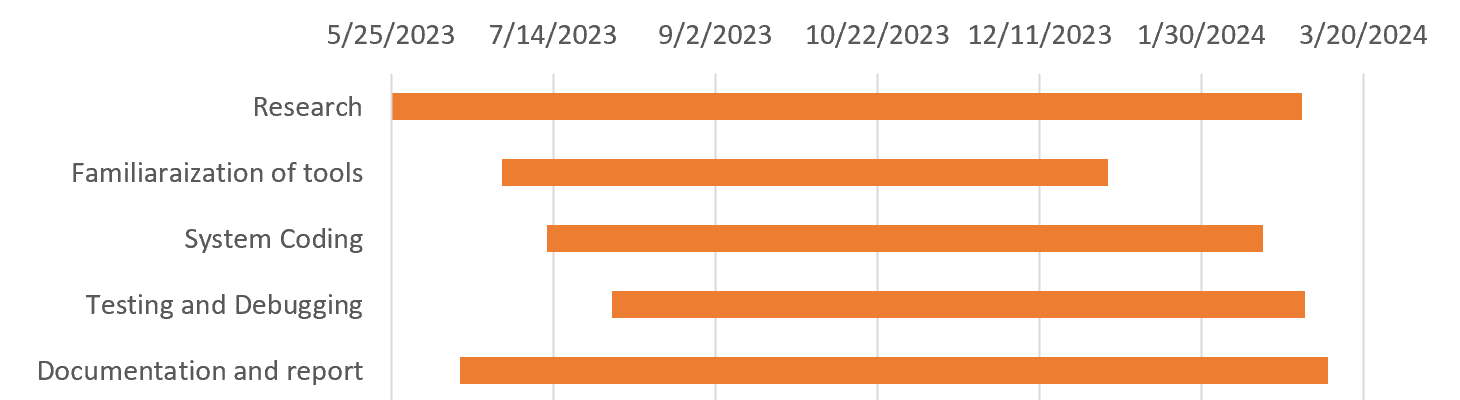
\includegraphics[scale=0.8]{images/Ganttchart.png}
    \caption{Gantt Chart}
    \label{fig:my_label}
\end{figure}



\chapter{Literature Review}
\section{Related Research}

	The proposed model for Nepali speech recognition combines CNN, GRU, and CTC networks with MFCC feature extraction, showing promising potential for accurately transcribing spoken Nepali speech into written text	 \cite{bhatta2020nepali}. This technology has the capacity to enhance interaction with communication devices and improve communication across various fields. Although the model achieves an 11\% Word Error Rate (WER) using a dataset from Open Speech and Language Resources, further research and refinement are needed to enhance accuracy and real-world applicability. The 1D-CNN component captures high-level features from MFCC representations, while the GRU component, a type of recurrent neural network, excels in modeling sequential data, enabling the model to learn temporal dependencies and enhance recognition accuracy by capturing the context and structure of the Nepali language.
	\\
	\\
	This study introduces a novel approach for developing a Nepali speech recognition model by utilizing a CNN-GRU architecture \cite{joshi2022novel}. The Librispeech dataset is employed to collect the necessary training data, which is then subjected to preprocessing and feature extraction through the application of MFCC. The CNN-GRU model is leveraged for feature extraction and the construction of the acoustic model, while CTC serves the purpose of decoding. The evaluation of the proposed model is based on the Word Error Rate metric, which measures the accuracy of the transcribed text. The deep learning approach demonstrates substantial performance improvements in comparison to traditional methods by employing separate phonetic and linguistic constructs. The key components of the speech recognition system include front-end processing for feature extraction and model building, as well as back-end processing involving decoding using a lexicon and language model. In this study, MFCC is utilized for feature extraction, the CNN-GRU network is employed for acoustic modeling, and CTC is utilized for decoding. The MFCC features represent sequences of acoustic feature vectors, each capturing information from a small time window of the speech signal to address its non-stationarity. The neural network is trained on the available data to predict unseen data, with the CNN component summarizing and extracting useful features from the input, while the RNN component, in conjunction with CTC, contributes to the model building process.

This paper presents an end-to-end (E2E) deep learning model for automatic speech recognition (ASR) with a focus on transcribing Nepali speech into text. The model is trained and evaluated using the OpenSLR dataset, which provides audio and text data \cite{dhakal2022automatic}. During dataset preprocessing, silent gaps present at the beginning and end of the audio files are clipped to enhance data quality. Mel Frequency Cepstral Coefficients (MFCCs) are utilized as audio features to input into the model. To achieve optimal performance, a combination of Bidirectional Long Short-Term Memory (LSTM), ResNet, and 1D Convolutional Neural Network (CNN) architectures are explored and compared. Different variations of LSTM, GRU, CNN, and ResNet are trained and tested, with the Bidirectional LSTM paired with ResNet and 1DCNN yielding the best results. For loss calculation during training, the Connectionist Temporal Classification (CTC) approach is employed, and CTC beam search decoding is utilized for character prediction. The project achieves a character error rate (CER) of 17.06 percent, outperforming other sequential models when evaluated on the OpenSLR dataset, thereby demonstrating its superiority in terms of test accuracy.
\\
\\
This study presents the development of a speech recognition system capable of transcribing audio input into text format \cite{shrestha2021nepali}. The system utilizes a combination of the Long Short-Term Memory (LSTM) neural network and the Connectionist Temporal Classification (CTC) function. Performance evaluation based on the Word Error Rate (WER) metric reveals a WER of 40\% without the CTC layer, which improves to 34.3\% with the inclusion of CTC. The initial step involves extracting informative features from raw speech data. Subsequently, an acoustic model is generated, representing speech as a combination of different phonetic units. Over time, various methods have been employed to capture temporal audio data, with probabilistic approaches such as Hidden Markov Models (HMM) and Gaussian Mixture Models (GMM) utilized in the early stages of speech recognition. However, to address inherent issues such as gradient vanishing and bursting, recurrent neural networks have undergone advancements leading to the development of LSTM and GRU networks. The main stages of the automatic speech recognition (ASR) process encompass data preparation, feature extraction, model building, training, testing, and validation.
\\
\\
This paper introduces a new method of interacting with technical devices through lexical communication, leveraging voice assistants as a key technology \cite{subhash2020artificial}. Voice assistants, powered by AI, have the capability to recognize human speech and respond using integrated voices. The proposed voice assistant system described in this paper collects audio input from the microphone and converts it into text. The text is then processed using the Google Text-to-Speech (GTTS) engine to generate an audio file in the English language. The audio file is played back using the "play sound" package in the Python programming language. The underlying principle of this system is Automatic Speech Recognition (ASR), which involves the device capturing audio from the microphone as the source. The recorded speech waveforms undergo acoustic analysis at three different levels: acoustic, pronunciation, and language modeling.

\section{Related Works}

One of the popular ASR software for Nepali is the Nepali ASR system developed by the Center for Speech and Language Technology (CSLT) at the University of Colorado Boulder \cite{websiteColorado}. This system is designed to recognize Nepali speech and convert it into written text. It has been trained on a large amount of Nepali speech data to improve its accuracy.

The Kaldi toolkit, a well-established and widely recognized open-source framework, has been a significant contribution to the field of automatic speech recognition (ASR) \cite{githubkaldi}. Developed in September 2011 by researchers at the Johns Hopkins University, Kaldi has gained prominence in academic and industrial domains. Its comprehensive set of tools and libraries make it a flexible and powerful platform for building state-of-the-art ASR systems. As we undertake the development of an ASR model for the Nepali language, the existence of the Kaldi toolkit serves as a valuable reference, showcasing its effectiveness in leveraging established techniques and providing a foundation for successful ASR implementations.

The combination of CNN, GRU, and CTC employed in Nepali speech recognition yielded a relatively high word error rate of 11\% \cite{bhatta2020nepali}. Therefore, for evaluating the performance, we have adopted the character error rate as the metric like our base paper \cite{dhakal2022automatic}, which resulted in a rate of 17.06\%. To enhance the accuracy, we intend to leverage a wider training dataset from openslr, excluding numeric transcriptions and unnecessary silent gaps. This refined dataset will be used in conjunction with a hybrid architecture comprising BiLSTM, 1-D CNN, and ResNet.

Moving forward, we plan to incorporate a voice assistant feature by integrating the generated text from the ASR system. Additionally, as our project progresses and resources permit, we aim to explore the use of transformers, an alternative architecture to BiLSTM, to further enhance the accuracy of the ASR system.




\chapter{METHODOLOGY}

\section{Working Mechanism}

\begin{figure}[h]
\centering
    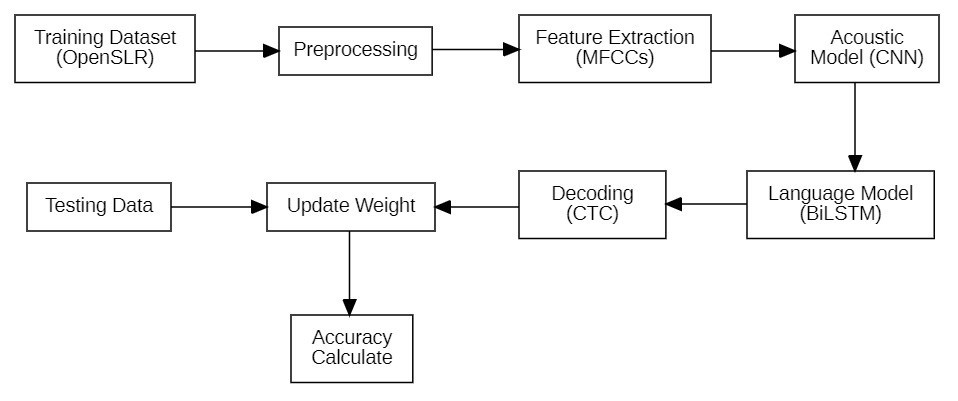
\includegraphics[scale=0.5]{images/Training Flowchart.jpg}
    \caption{Block diagram of the Proposed ASR Training Model}
    \label{fig:my_label}
\end{figure}

\begin{figure}[h]
\centering
    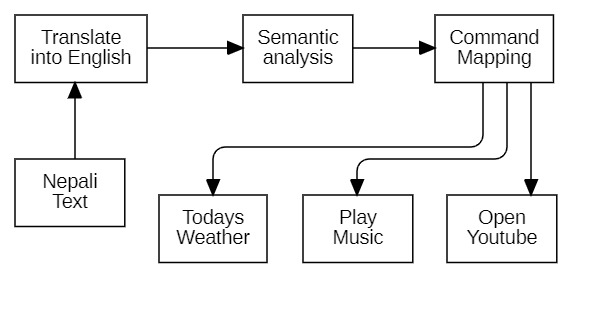
\includegraphics[scale=0.5]{images/Implementation Flowchart.jpg}
    \caption{Block diagram of the Proposed ASR Implementation }
    \label{fig:my_label}
\end{figure}
\begin{enumerate}
	\item Dataset:  Two potential datasets will be used: High quality TTS data for Nepali (openslr.org/43)\cite{kjartansson-etal-tts-sltu2018} and Large Nepali ASR training dataset (openslr.org/54) \cite{kjartansson-etal-sltu2018}. The first dataset contains female transcribed audio data for the Nepali language. It includes 2064 high-quality audio files from 18 different speakers, with multiple audio files per speaker having similar word and character patterns. However, the vocabulary and text sequences might not be diverse, leading to potential bias in the ASR model's predictions if used. On the other hand, the second dataset provides significant advantages with a larger vocabulary, more speakers, a greater number of audio files, and a more diverse sequence of characters and text. This dataset will be used for training and testing the ASR model. It consists of 157,905 audio clips from 527 unique speakers, sampled at 16KHz. The dataset will be sourced from OpenSLR, a platform hosting speech and language resources for speech recognition. Before training, an initial cleansing process will be performed on the dataset by eliminating numeric transcriptions to prevent degradation of the model's overall performance. After removing these instances, approximately 143.6 hours of 148,188 audio clips will remain as the foundation for training and testing the model.

	\item Preprocessing: The dataset will be acquired using OpenSLR, which will provide a collection of speech and language resources. Firstly, the dataset will undergo a cleansing process to eliminate numeric transcripts, as this type of data will play a minimal role and degrade the overall performance of the model. The majority of the dataset will contain large silent gaps, so the silent gaps will be clipped. This process will make the data more suitable for feature extraction and further processing, reducing potential errors.
	\\
	ALGORITHM 1: Clipping of silent gaps from both ends
	\\
	\begin{quote}
	wav $\gets$ sampled audio signal
	\\
    $\Delta$  $\gets$ appropriate window length
    
\textbf{INPUT}: wav,$\Delta$
\\
\textbf{PROCESS}:
\\
wavAvg $\gets$ Average( $\left| wav \right|$)
\\
N $\gets$ Length(wav)
\\
\\
/* Removing the silent gap from the start */
\\
\textbf{for} idx = 0, $\Delta$ , 2 $\Delta$ , . . . ,N - $\Delta$ \textbf{do}
\\
\hspace*{1cm} win $\gets$  wav[ idx : idx + $\Delta$  ]
\\
\hspace*{1cm} winAvg ← Avergae($\left| win \right|$)
\\
\hspace*{1cm} \textbf{if} $winAvg > wavAvg$ then
\\
\hspace*{2cm}wav ← wav[idx :]
\\
 \hspace*{2cm}\textbf{break}
 \\
 \hspace*{1cm} \textbf{end if}
 \\
 \textbf{end for}
 \\
 \\
 /* Removing the silent gap from the end */
 \\
\textbf{for} idx = N - $\Delta$, N - 2 $\Delta$, . . . , 0 do
\\
\hspace*{1cm} win ← wav[idx : idx + $\Delta$]
\\
\hspace*{1cm} winAvg ← Avergae($\left| win \right|$)
\\
\hspace*{1cm} \textbf{if} $winAvg > wavAvg$ then
\\
\hspace*{2cm} wav ← wav[: idx]
\\
\hspace*{2cm} \textbf{break}
\\
\hspace*{1cm} \textbf{end if}
\\
\textbf{end for}
\\
\textbf{OUTPUT}: processed\textunderscore wav ← wav
\end{quote}





	\item  Feature Extraction: The extraction of the best parametric representation of acoustic signals will be an important task to produce better recognition performance. Mel Frequency Cepstral Coefficients (MFCCs) will be a powerful feature extraction mechanism that will generate coefficients [6]. This feature extraction mechanism will go through six stages:
	\\
	\begin{itemize}
	
 \item Pre-emphasis: The signal will be processed through a filter that emphasizes higher frequencies, increasing the energy of the signal at higher frequencies.
\item Framing: The speech samples obtained will be segmented into smaller frames.
\item Windowing: Samples will be multiplied using a scaling function to smooth the signals near the edges.
\item Discrete Fourier Transform(DFT): Each frame's samples will be converted from the time domain into the frequency domain.
\item Mel Filter Bank Processing: The frequency range in the DFT spectrum is very large and wide. Mel filter banks will have a collection of bandpass filters over the mel scale. The FFT signal obtained will pass through the Mel scale filter bank, and each filter's output will be the sum of its filtered spectral components.
\item Discrete Cosine Transform(DCT):  The log Mel spectrum obtained through Mel filter bank processing will be converted into the time domain using DCT. The result of this conversion will be called Mel Frequency Cepstral Coefficients (MFCCs). MFCCs will be highly favorable for signal processing with RNN, DNN, and CNN. For human speech, 13 mel scales will be sufficient for extracting features from the signal. The equation involved in calculating the mel scale from the frequency in Hertz (f) will be given by
\begin{quote}
 \label{eq:mel}
                  \hspace{3cm}                              \text{Mel}(f) = 2595*log(1+(f/700))  \hfill (1)
\end{quote}
\begin{figure}[h!]
    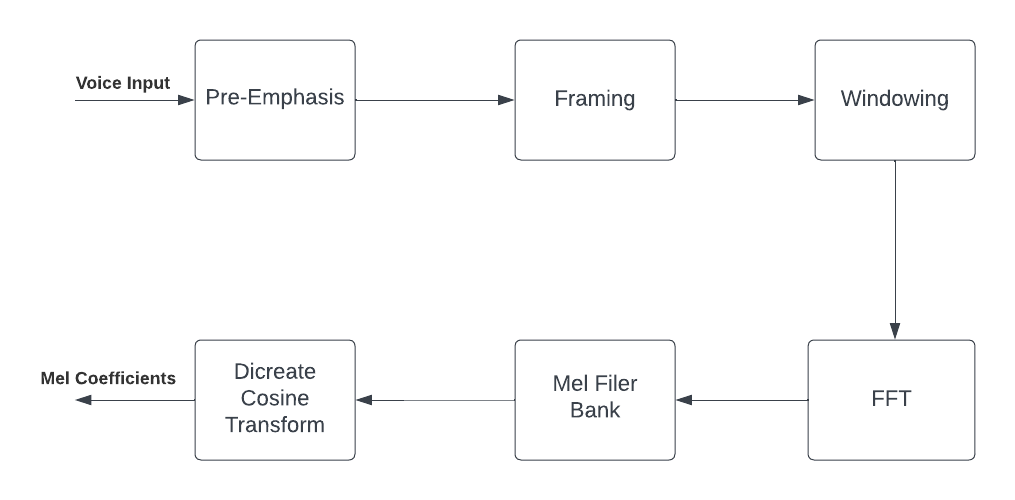
\includegraphics[scale=0.4]{images/BlockMFCC.png}
    \caption{Block Diagram of MFCC}
    \label{fig:my_label}
\end{figure}
\end{itemize}


	\item  Acoustic and Language Model:
	\begin{itemize}
	
	
\item  Residual Block(ResNet): 
 The ASR Model will begin with the implementation of Residual Blocks. These blocks will utilize shortcut connections to add the input of a block into the output of our stacked layers. The residual block for our model will have an output of G(x)+x, where x will be the block's input and G(x) will be the output of stacked layers.
\item   1D-CNN: After residual blocks, the model will employ a 1D-CNN layer for localized feature extraction. The 1D-CNN will perform convolution operations on the temporal direction of the signal and will use trained weighted filters (kernels) to extract localized features. This process will help extract relevant features from the input audio.
\item  Batch Normalization(BN): The output of the 1D-CNN layer will be passed through batch normalization. BN will normalize the output vector by using the mean and variance from the current batch. It will add stability and speed to the gradient descent process during model training.
\item   Parametric ReLU:  The normalized values from the BN layer will then be passed through the Parametric ReLU (PReLU) activation function. PReLU will introduce non-linearity to the model by applying a rectified linear function with learnable parameters.
\item  Residual Learning: The output of the PReLU function will be added to the input of the residual block, creating a residual learning mechanism. This will allow the model to learn residual information and make improvements based on the difference between the input and output.

\begin{figure}[h!]
\centering
    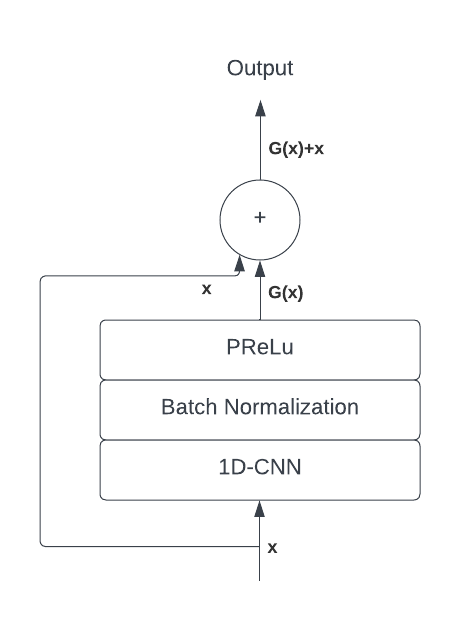
\includegraphics[scale=0.8]{images/residuallearning.png}
    \caption{Diagram of Residual Learning}
    \label{fig:my_label}
\end{figure}
\item  RNN Layers: The output of the last residual block will serve as input to the stacked RNN layers (mainly BiLSTM). RNN will be a neural network that will use the previous time step's output as input for the current time step. RNNs will be suitable for sequential data and will be able to capture contextual information over time. The RNN layers will provide multiple levels of feature abstraction to generalize patterns in the data. Mainly, Bidirectional Long Short-Term Memory (BiLSTM) will be a variant of RNN used in our model. It will process the input sequence in both forward and backward directions simultaneously, capturing information from past and future contexts. 
\\
Multiple BiLSTM layers can be stacked together to capture complex dependencies. It will enhance the ASR model's ability to understand and transcribe speech data accurately.
\item   Dense Layers and Softmax Output: The output of RNN layers (i.e., BiLSTM layers) will be fed into the dense layers of the neural network, which will further process the features learned by RNNs. Finally, a softmax layer will be applied to obtain a probability distribution over the 66 unique characters. The softmax output can be represented as:
Softmax\textunderscore output = Softmax(Dense(RNN\textunderscore output))
\item  CTC(Connectionist Temporal Classification) Loss: The CTC loss function will be used to compare the softmax output with the targeted transcriptions. The CTC loss will help handle the alignment problem between input audio and output characters. It will compute an alignment-free loss value using a blank token introduced during training and inference. The CTC loss can be calculated as:
CTC\textunderscore loss = -log(p($Y|X$))   , where p($Y|X$) will represent the probability of the target transcription Y given the input audio X.

And, The objective function(i.e Probability p($Y|X$) will be the sum of all possible valid sequences. 
Mathematically,  
\begin{quote}
                  \hspace{3cm}    p($Y|X$)=$\Sigma$ \textsubscript {$A \in A $ \(x_,y\)} * {$\Pi$ \textsuperscript T \textsubscript{t=1}}p \textsubscript{t} ($a \textsubscript{t}|X$) \hfill (2)
\end{quote}
where A\(x_,y\) will be the valid alignment of Y given X.
\end{itemize}



	
		\item  Decoding Algorithm: During prediction, the softmax outputs will need to be decoded to obtain a sequence of characters. The CTC beam search decoding method will be used in our model. CTC Beam Search will consider multiple alignments at each time step and will find the most probable output sequence. The process will involve tokenization, beam initialization, expansion, scoring, and pruning to select the final sequence. CTC Beam Search will effectively address the challenge of aligning audio inputs with output characters, resulting in accurate and contextually coherent transcriptions.
		\begin{figure}[h!]
\centering
    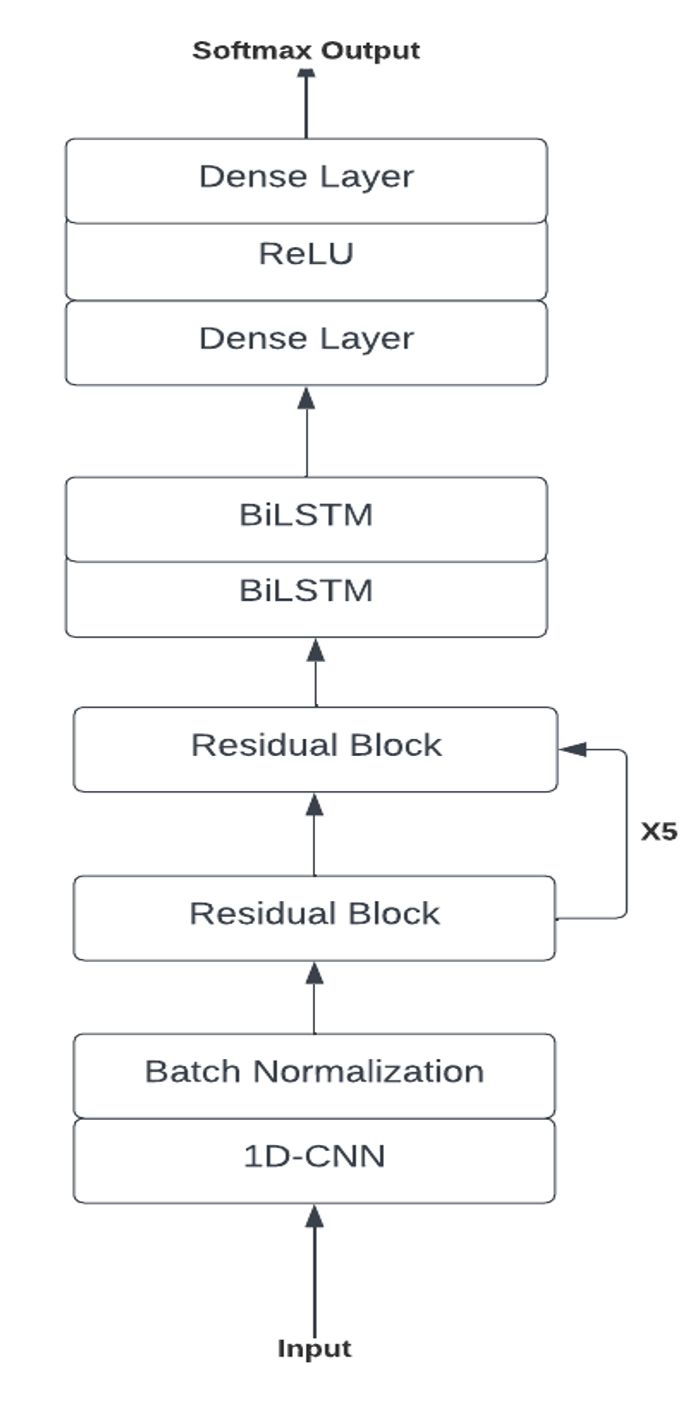
\includegraphics[scale=0.8]{images/decoding.png}
    \caption{Diagram of  ASR Model}
    \label{fig:my_label}
\end{figure}
\newpage
	\item  Transcription Output:At the last stage of ASR modeling, the output text of the given speech/voice input will be obtained.
	\item Language Translation and Commanding: We will utilize the Nepali text received from ASR (Automatic Speech Recognition) as input for Google Text To Speech (GTTS) to translate it into English. This translation process will be facilitated by the GTTS API, which we will employ for this purpose.
	\item Semantic analysis and command mapping: Different expressions can be used to convey the same meaning. In this case, we will utilize the semantic analysis functionality of the Google API to associate those variations with specific actions. For example, commands such as "open YouTube," "play music," or "perform calculations" will be mapped to their respective tasks using the semantic analysis feature.
	
\end{enumerate}
\newpage
\section{\ac{UML} Diagrams}
\subsection*{Use Case Diagram}
\begin{figure}[h!]
    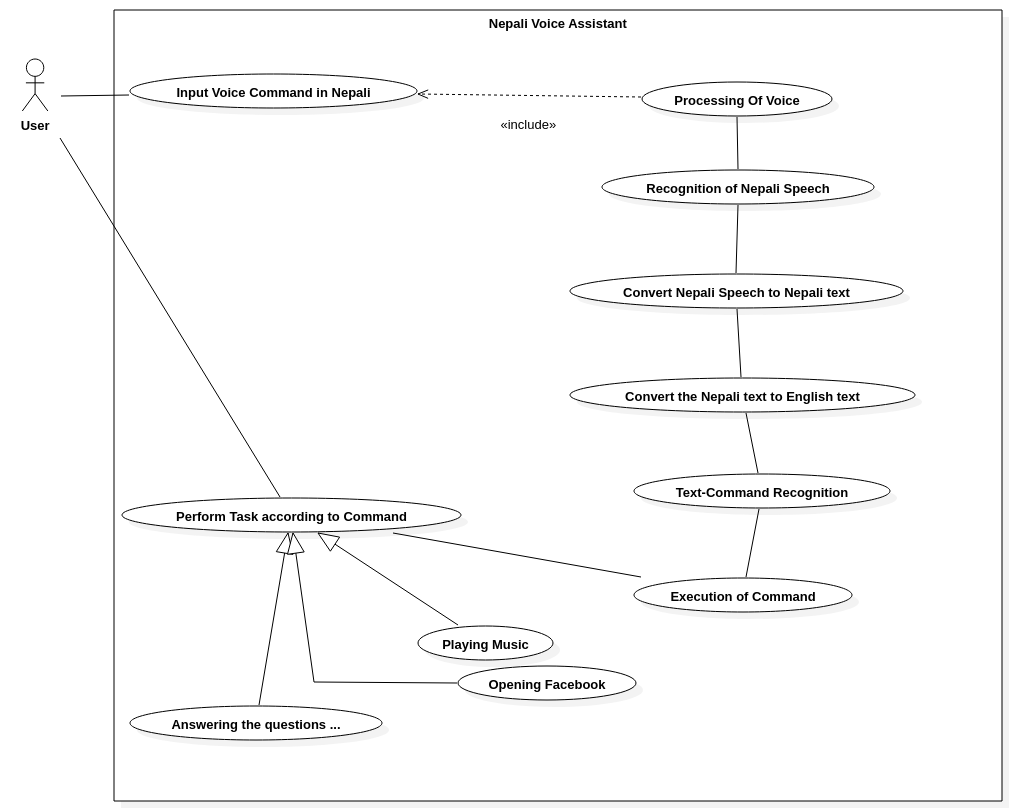
\includegraphics[scale=0.45]{images/usecase.png}
    \caption{Use Case Model of the Proposed System}
    \label{fig:my_label}
\end{figure}
\newpage
\subsection*{Activity Diagram}
\begin{figure}[h]
	\centering
    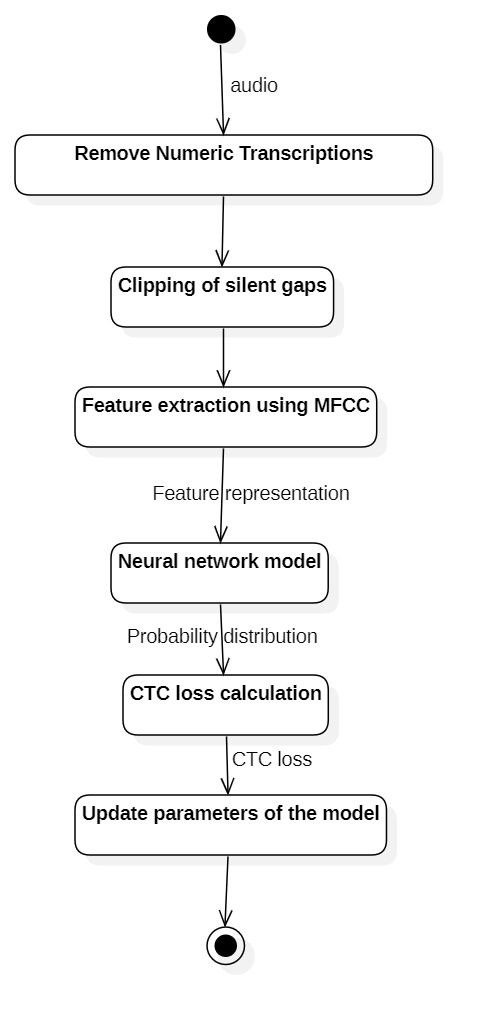
\includegraphics[scale=0.5]{images/ActivityDiagram1.jpg}
    \caption{Activity Diagram of the Proposed System}
    \label{fig:my_label}
\end{figure}
\newpage



\section{Software Development Model}
The incremental model is one of the easiest software development life cycle models to implement. It is suitable for scenarios where the initial or core software requirements are clearly defined, but the full set of features for the project is unknown. Additionally, the development company may choose not to provide the complete functionality of the software at once, but instead opt for periodic updates. Alternatively, clients may request functionality enhancements during the development process. In such cases, the incremental model is utilized.
\\
\\
\begin{figure}[h]
    \centering
    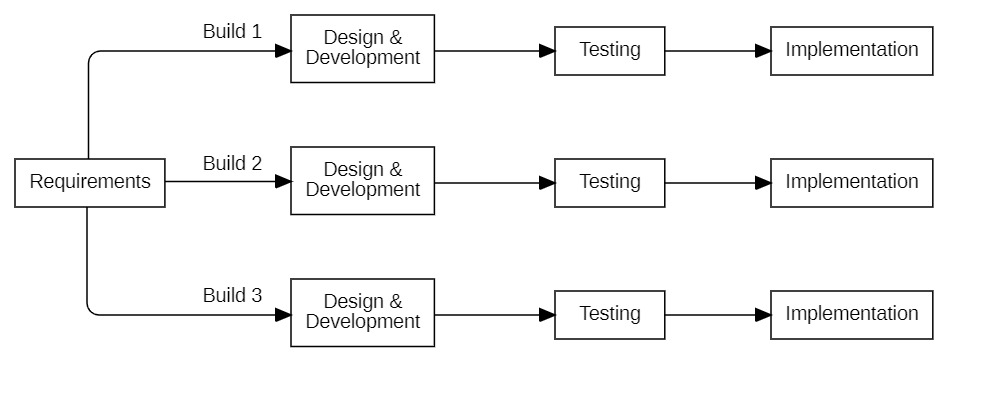
\includegraphics[scale=0.4]{images/incremental.jpg}
    \caption{Incremental Model}
    \label{fig:my_label}
\end{figure}
\begin{itemize}
\item Build 1: In the initial phase, we proceed to utilize the voice input . This input is then processed using Automatic Speech Recognition (ASR) technology to convert it into text written in Nepali, conveying the equivalent meaning.
\item Build 2: In the subsequent phase, we will take the Nepali text obtained as input from ASR and proceed to convert it into English text using the Google API. Additionally, we employ the Google API's semantic analysis feature to accurately associate the command with the corresponding task.
\item Build 3: For the final version, we will create a desktop interface that includes the functionality to accept user voice as input for our system. Additionally, the interface will display the corresponding translated text for the user's input.
\end{itemize}



\chapter{EPILOUGE}

\section{Expected Output}
The expected output of Nepali speech recognition entails the accurate transcription of spoken Nepali language into written text. When using an Automatic Speech Recognition (ASR) system designed for Nepali, the system is expected to capture the words, phrases, and sentences spoken in Nepali with a high degree of accuracy. This ensures that the transcribed text reflects the intended message accurately. After that we will use the text obtained in Nepali representation for our voice assistant .

\section{Work Completed}
We have implemented the conversion to MFCCs coefficient created by removing silent gaps and removing the unwanted devnagari transcription. Furthermore, we have written the code to implement the ASR model and Residual Block. The dataset we are using to train is taking excessive amount of time due to which we have just taken a sample of 44 audio files with epoch 10, the corresponding transcription to see the working of the model, plus taking 80\% of dataset for training and 20\% for test set.  

\section{Work Remaining}
The Build 2 and Build 3 part are the remaining part, plus the training with much larger dataset to improve the accuracy must be done .






\newpage
%Reference
\renewcommand\bibname{REFERENCES} % Change heading to References
\bibliographystyle{IEEEtran} % to use IEEE Format for referencing
\addcontentsline{toc}{chapter}{References} % to add references in TOC
\bibliography{library} % specify the .bib file containing reference information 






%Comment this Chapter if you do not need to include Appendix.

%\addcontentsline{toc}{chapter}{Appendix}



	
\end{document}
